\section{Negocio}
\subsection{Introducción}

En el apartado de negocio se presenta el modelamiento de los procesos de negocio que son desarrollados dentro de la organización, permitiendo un mayor entendimiento de cada factor que actua en la organización.

\newpage

\subsection{Punto de Vista de Organización}

El punto de vista de la organización permite identificar los actores, roles y colaboraciones que interactuan en la organización.

%%grafo

\begin{figure}[th!]
	\centering
	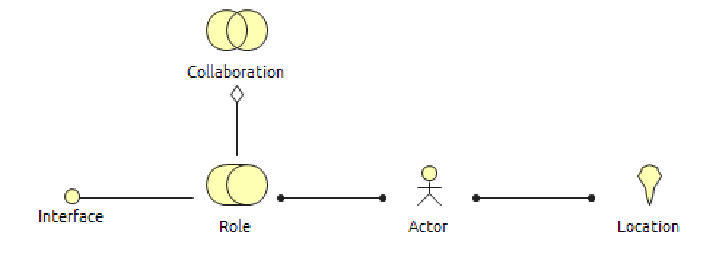
\includegraphics[width=13cm,height=6cm]{arquitectura/negocio/imgs/m_organizacion}
	\caption{Modelo de Organización}{\scriptsize \textbf{Fuente:} Archimate 2.0}
\end{figure}

\subsection{Caso}

En la organización que se presenta dentro de las propiedades horizontales se puede ver roles muy bien definidos.

%%grafo
\begin{figure}[th!]
	\centering
	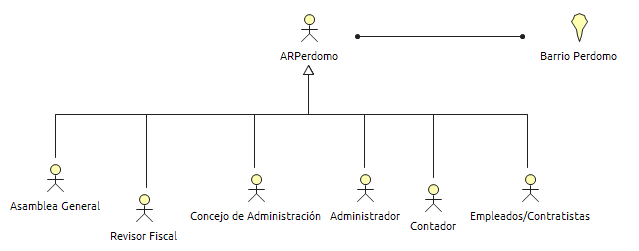
\includegraphics[width=12cm,height=7cm]{arquitectura/negocio/imgs/organizacion}
	\caption{Caso de Organización}{\scriptsize \textbf{Fuente:} Imagen propia}
\end{figure}
\newpage

\subsection{Punto de Vista de Función de Negocio}

La función de negocio permite determinar las tareas que debe realizar cada rol

%%grafo

\begin{figure}[th!]
	\centering
	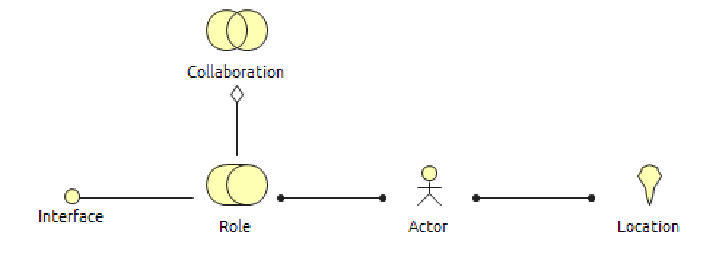
\includegraphics[width=12cm,height=7cm]{arquitectura/negocio/imgs/m_organizacion}
	\caption{Modelo de Organización}{\scriptsize \textbf{Fuente:} Archimate 2.0}
\end{figure}

\newpage
\subsection{Caso}

En el punto de vista presentado a continuación se reflejan las funciones de cada roles, especificando las labores que de cada uno de ellos.

%%grafo
\begin{figure}[th!]
	\centering
	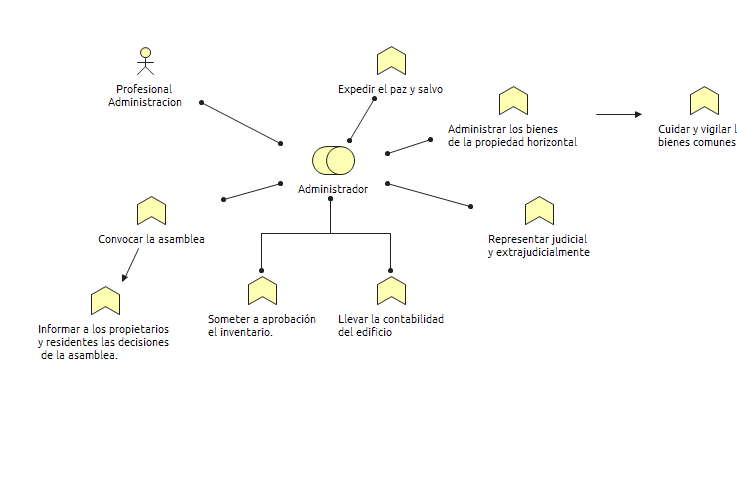
\includegraphics[width=13cm,height=8cm]{arquitectura/negocio/imgs/funciones-1}
	\caption{Funciones administrador}{\scriptsize \textbf{Fuente:} Imagen propia}
\end{figure}


\begin{figure}[th!]
	\centering
	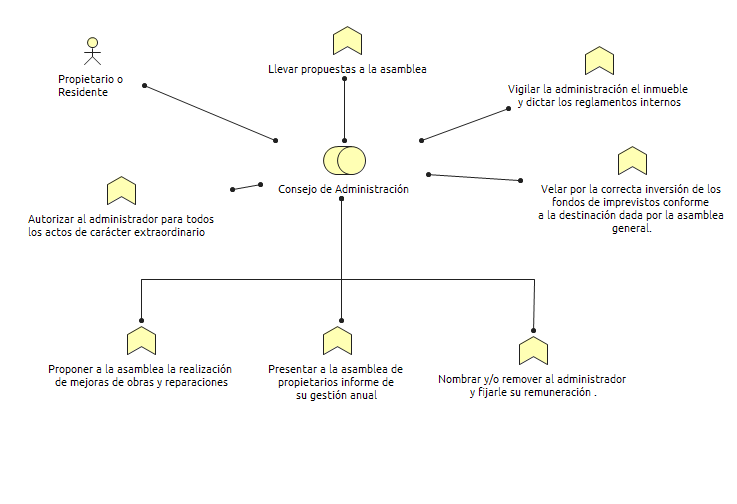
\includegraphics[width=13cm,height=8cm]{arquitectura/negocio/imgs/funciones-2}
	\caption{Funciones consejo administrativo}{\scriptsize \textbf{Fuente:} Imagen propia}
\end{figure}
\begin{figure}[th!]
	\centering
	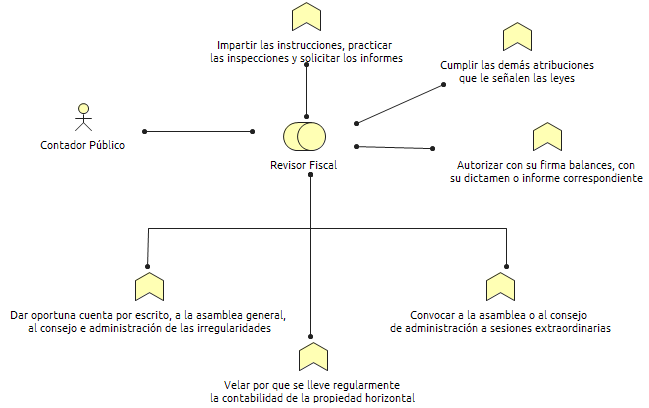
\includegraphics[width=13cm,height=8cm]{arquitectura/negocio/imgs/funciones-3}
	\caption{Funciones revisor fiscal}{\scriptsize \textbf{Fuente:} Imagen propia}
\end{figure}
\newpage

\subsection{Punto de Vista de Proceso de Negocio}
descripción

%%grafo

\begin{figure}[th!]
	\centering
	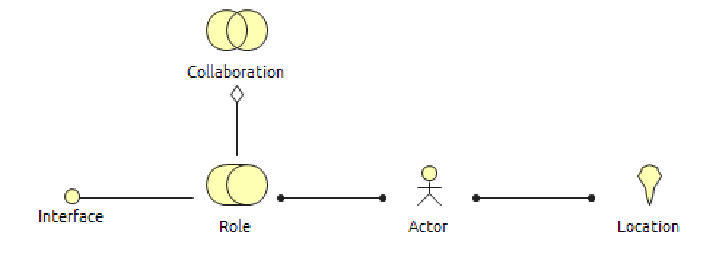
\includegraphics[width=12cm,height=7cm]{arquitectura/negocio/imgs/m_organizacion}
	\caption{Modelo de Organización}
\end{figure}

\newpage
\subsection{Caso}
descripción

%%grafo
\begin{figure}[th!]
	\centering
	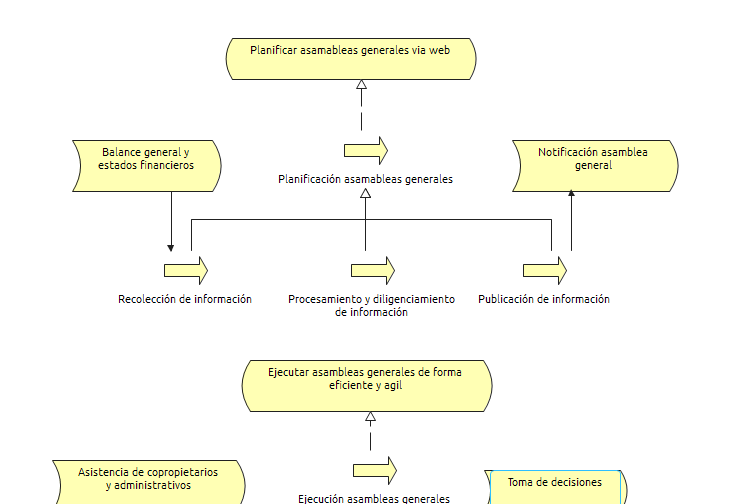
\includegraphics[width=12cm,height=7cm]{arquitectura/negocio/imgs/proceso}
	\caption{Proceso de negocio}
\end{figure}
\newpage

\subsection{Punto de Vista de Cooperación de Proceso de Negocio}
descripción

%%grafo

\begin{figure}[th!]
	\centering
	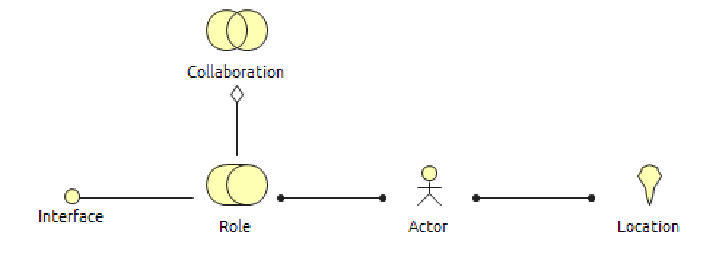
\includegraphics[width=12cm,height=7cm]{arquitectura/negocio/imgs/m_organizacion}
	\caption{Modelo de Organización}
\end{figure}

\newpage
\subsection{Caso}
descripción

%%grafo
\begin{figure}[th!]
	\centering
	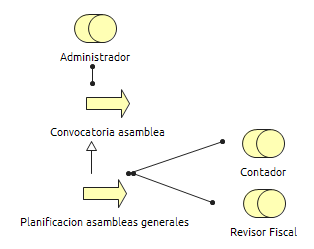
\includegraphics[width=12cm,height=7cm]{arquitectura/negocio/imgs/cooperacion-proceso}
	\caption{Cooperación de proceso de negocio}
\end{figure}
\newpage

\subsection{Punto de Vista de Producto}
descripción

%%grafo

\begin{figure}[th!]
	\centering
	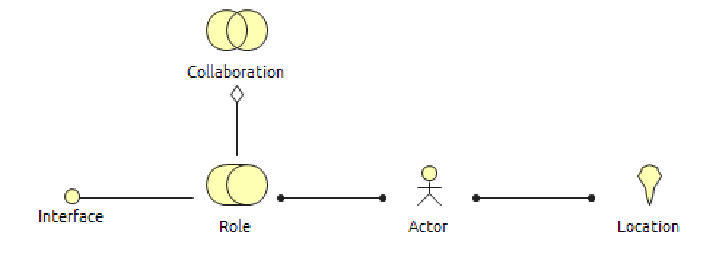
\includegraphics[width=12cm,height=7cm]{arquitectura/negocio/imgs/m_organizacion}
	\caption{Modelo de Organización}
\end{figure}

\newpage
\subsection{Caso}
descripción

%%grafo
\begin{figure}[th!]
	\centering
	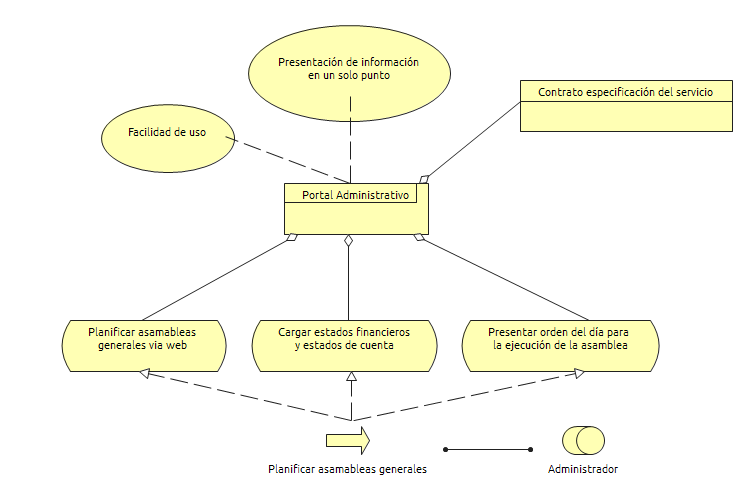
\includegraphics[width=12cm,height=7cm]{arquitectura/negocio/imgs/producto}
	\caption{Producto de negocio}
\end{figure}
\newpage